\documentclass[../main.tex]{subfiles}
\graphicspath{{\subfix{..}}}

\begin{document}
\chapter{Reliability of machine learning methods}
\label{sec:janne}

\epigraph{``Psychohistory was the quintessence of sociology; it was the science of human behavior reduced to mathematical equations. The individual human being is unpredictable, but the reactions of human mobs, Seldon found, could be treated statistically''}{Isaac Asimov, Second Foundation}

\minitoc

As explained in previous chapters, JUNO is a precision experiment where the complete understanding of the effects at hand is crucial. As it will be illustrated in chapter \ref{sec:joint_fit}, even small invisible biases or uncertainties could lead to the imposibility to run the measurements, or even worse, wrong our mass ordering measurements. While the liquid scintillator technology is well none and straightforward, this is the first time it is deployed to such scale, and for such precision. This novelty bring its fair share of elements, effects or assumption, that, if they were to be overlooked, could cause issue.

We already shown a large variety of reconstruction algorithms, OMILREC for LPMT reconstruction in section \ref{sec:juno:reco}, numerous machine learning algorithms in section \ref{sec:juno:ml} and our own work in chapters \ref{sec:jcnn} and \ref{sec:jgnn}. Those algorithms were compared to each others based on their performance as in \cite{qian_vertex_2021} but we are the first that looked into the correlation between the reconstruction. The combinations of algorithms shown in chapter \ref{sec:jcnn} and chapter \ref{sec:jgnn} show that some information elude the algorithms. We used this fact to try to improve our performance but this could also lead the algorithm to being vulnerable to some effect that could affect the detector and wrong the measurements.

The search for such effect could be done by hand, but the process would be tedious. We propose in this thesis a machine learning method to probe for those effects. In section \ref{sec:janne:motivation}, I delve further in the motivations of this work. In section \ref{sec:janne:method}, I describe the method behind the algorithm. In section \ref{sec:janne:arch} I detail the architecture of our algorithm and in section \ref{sec:janne:results} the results of it. Finally, in section \ref{sec:janne:conclusion}, I conclude and dicuss about the prospect and possible improvements to bring to this work.

\section{Motivations}
\label{sec:janne:motivation}
%\begin{itemize}
%  \item JUNO needs very good understanding of reconstruction
%  \item Estimator combination shows that there can be improvement due to simplfication and that NN/reco methods can have hard time grasping all the detector effect.
%  \item If there is potential failure point, we need to search for them
%  \item La mesure de la NMO est tres sensible (see $alpha_{qnl}$ joint fit chapter)
%\end{itemize}

As introduced above, JUNO needs a very good understanding of the biases and effects affecting its reconstruction as a small bias could wrong the mass ordering measurement. To calibrate those biases and effect, JUNO rely on multiples sources that will be located at various point in the detector. The calibration strategy was already discussed in section \ref{sec:juno:calib} and show calibrations sources of gammas, neutrons and positrons, with the catch that the positrons will annihilate inside the encapsulation and only the two 511 keV gammas will be seen. All those sources will be located at the center of the detector, impervious to non-uniformity.

A second, natural, source will be used for calibration: The $^{12}B$ spectrum. The $^{12}B$ is a cosmogenically produced isotope through the passage of muons inside the LS. The $^{12}B$ decays via $\beta^-$ emissions with a Q value of 13.5 MeV with more than 98\% of the decay resulting in ground state $^{12}C$. The $^{12}B$ event will be cleanly identified by looking for delayed high energy $\beta$ events after an energetic muon. Due to its natural causes, the $^{12}B$ events will be uniformly distributed in the detector. The calibration strategy consist in fitting the energy spectrum of $^{12}B$ with the results of the simulation to adjust the simulation parameters.

We see that, while the calibration strategy is pretty complete, its missing a few points. First, none of the calibrations sources considered are positrons. While electrons and positrons events should be pretty similar in their interaction with the electronic cloud of the LS atoms, electron events are missing the two annihilations $\gamma$ and the potential of forming a positronium \cite{schwarz_measurements_2018}. The topology of the event thus differ of the order of magnitude of our reconstruction performance, a few nanoseconds for the energy deposit and positronium annihilation against a time transit spread between 3 and 6 ns depending on the PMT type \cite{rodphai_20-inch_2021, liao_study_2017, li_characterization_2018} and the $\gamma$ will travel distances of the order of magnitude of the typical LPMT resolution of 8 cm (see section \ref{sec:juno:reco}). Moreover, where for calibration sources the localization will be well known, the individual truth of $^{12}B$ will be unknown. We thus need to compare our model to higher order observables such as energy distribution more than individual comparison.

If there is potential failure point in those considerations, we need to search for them efficiently.

\section{Method}
\label{sec:janne:method}
%\begin{itemize}
%  \item Slide benoit
%    \begin{itemize}
%      \item En gros: Chercher de potentiels erreurs dans la reconstruction qui serait invsible à la calibration et control samples
%      \item Possible car pas de sources positron pour la calibration
%      \item Certaines techniques de calibrations sur base sure des variables de haut niveau (moyenne, fit de spectre, etc...) de par l'impossibilité d'acceder à la vérité vrai de ces evenements de calibration
%    \end{itemize}
%\end{itemize}

All of the considerations could hide potential unknown or undetected effect that could lead to issue in the mass ordering analysis. But, while we have idea from where the issue could come, the production by hand of event perturbations that would not show in the calibration would be tedious. That's why we propose to use a Neural Network to produce those perturbations if they exists. A schematic of the concept is presented in figure \ref{fig:janne:method:schema}.

\begin{figure}[ht]
  \centering
  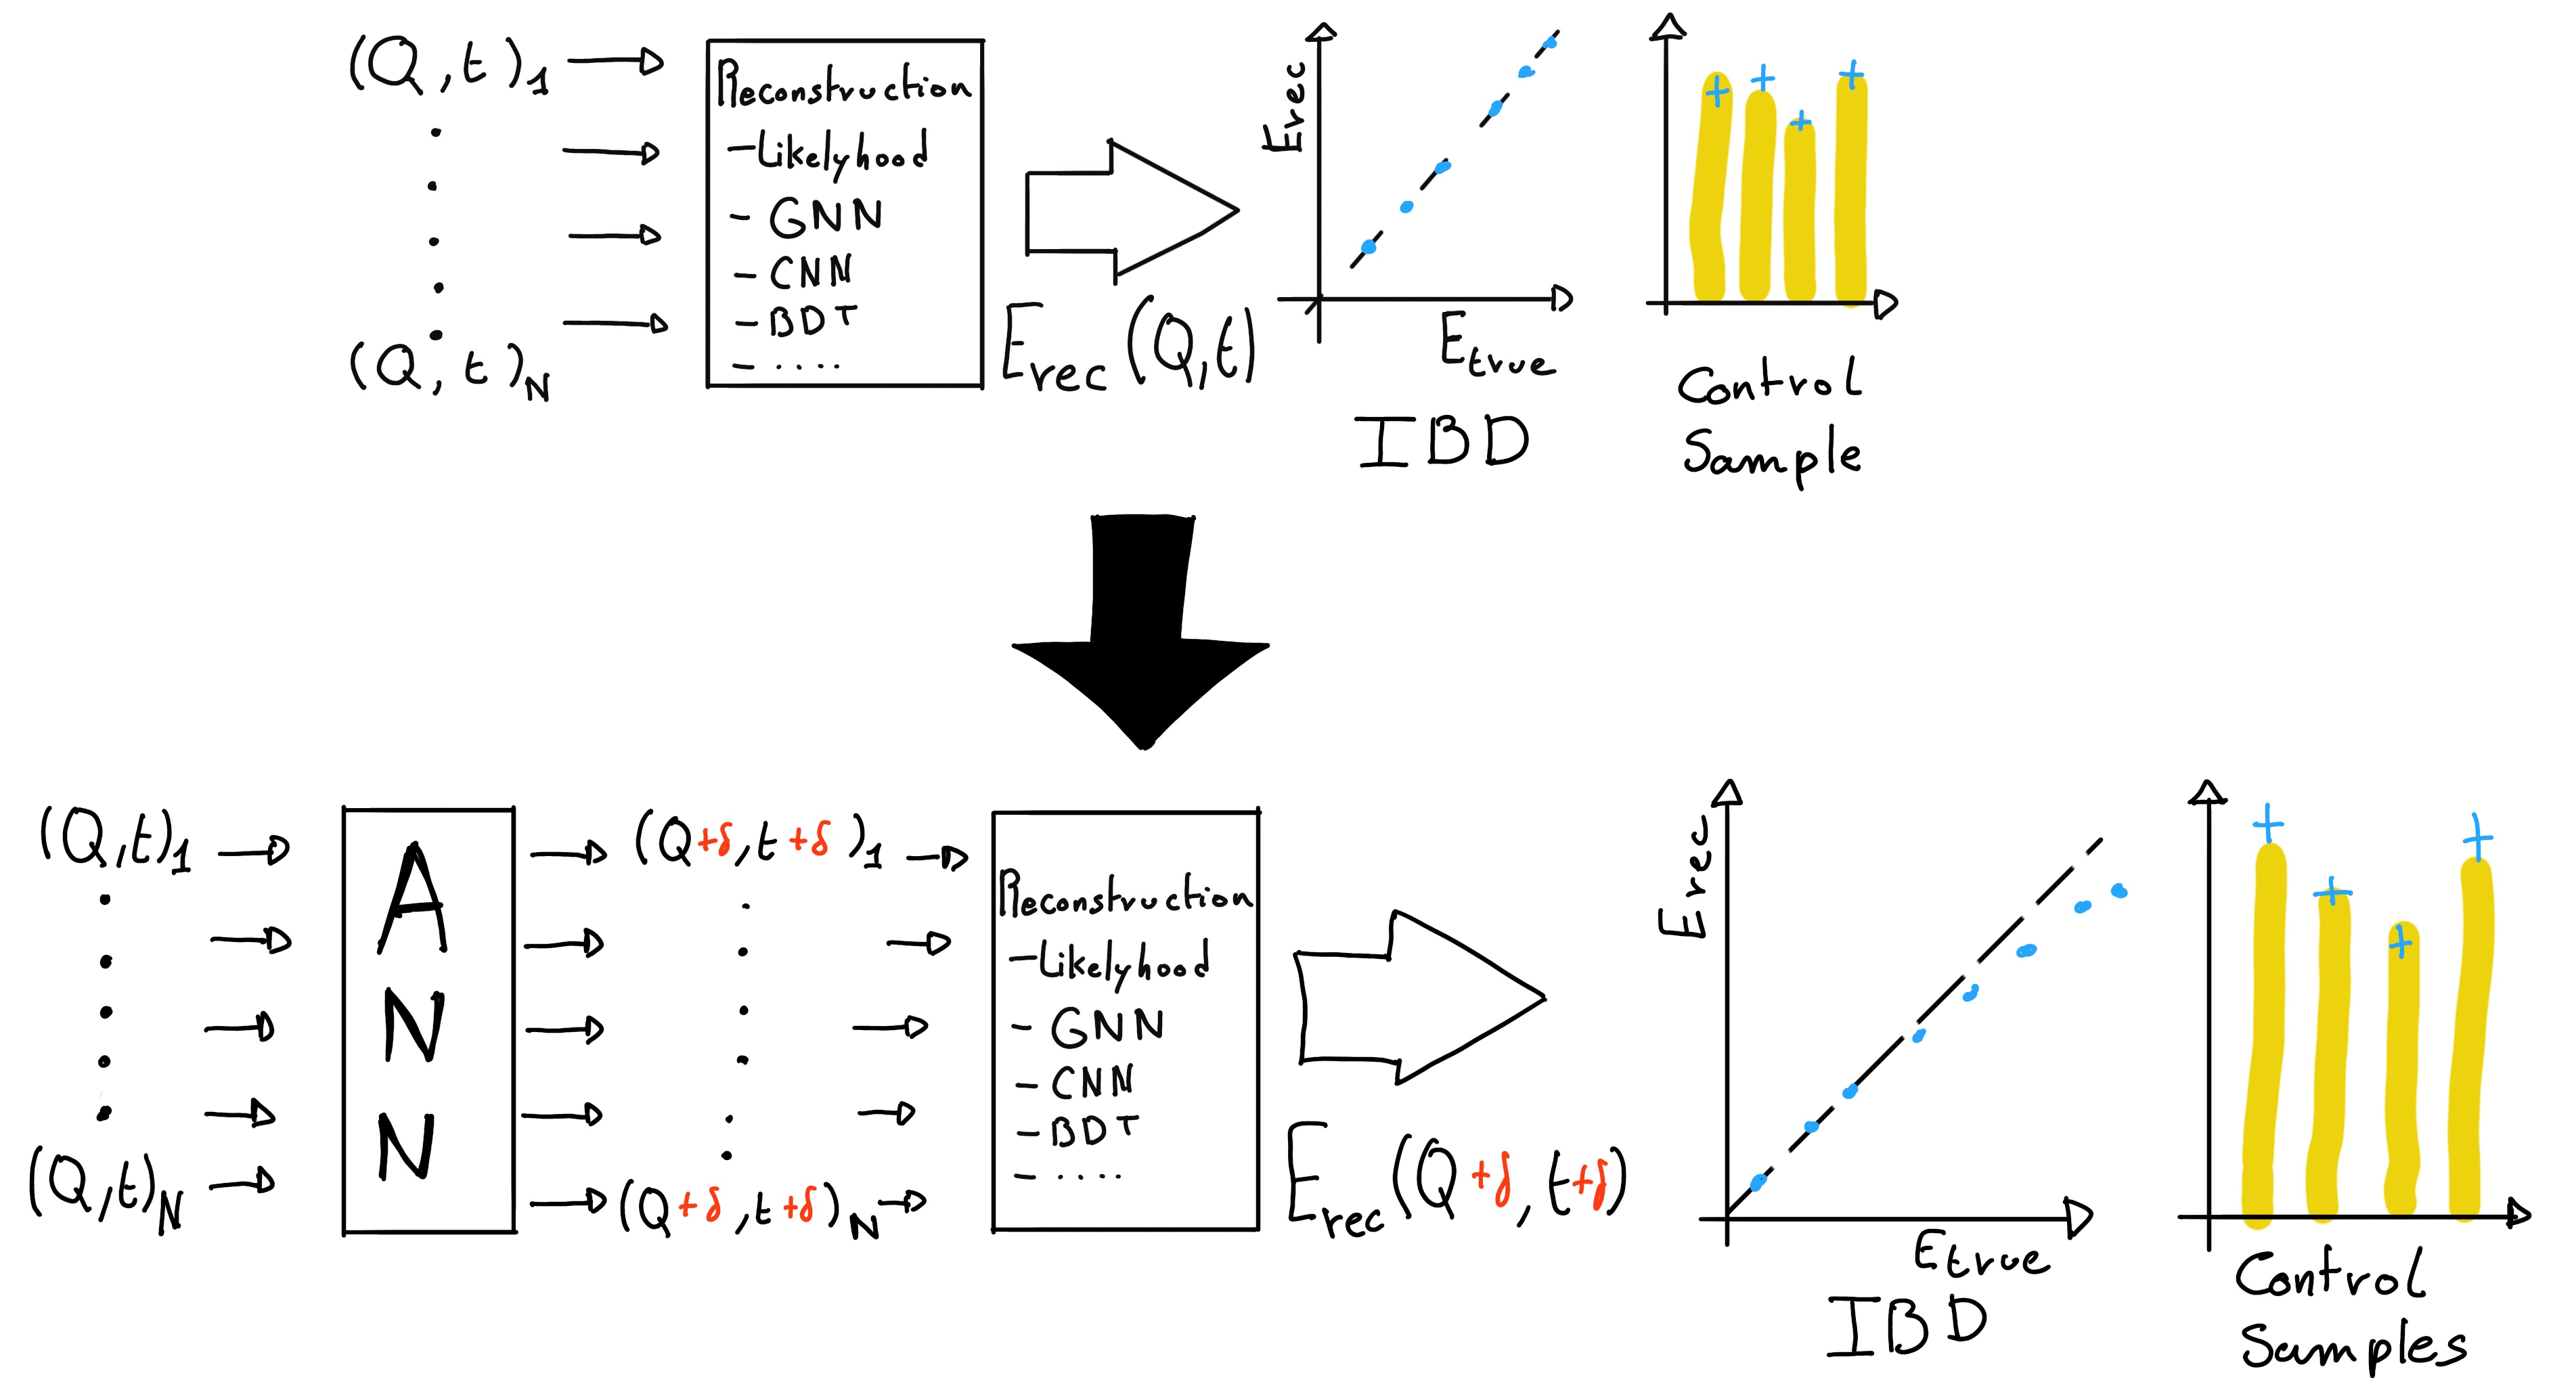
\includegraphics[width=\linewidth]{images/janne/ann_method.jpg}
  \caption{Schema of the method to discover vulnerabilities in the reconstruction methods}
  \label{fig:janne:method:schema}
\end{figure}


\section{Architecture}
\label{sec:janne:arch}
\begin{itemize}
  \item Expliquer la problematique dans l'architecture
  \item Ambition de pouvoir etre appliqué a toutes les methodes, pas que NN
  \item Pb techique: descente de gradient
  \item Présenter la loss
\end{itemize}

\subsection{Adversarial Neural Network}
\label{sec:janne:arch:ann}
\begin{itemize}
  \item Decrire l'architecture de l'ANN
\end{itemize}

\subsection{Reconstruction Network}
\label{sec:janne:arch:reco}
\begin{itemize}
  \item Reseau de Neurone Simple. Deux avantages:
  \item Besoin pour la descente de gradient
  \item Un reseau "simpliste" a plus de chance de présenter des "défauts" que l'ANN pourrait exploiter
\end{itemize}

\subsection{Training}
\label{sec:janne:arch:training}
\begin{itemize}
  \item Presentation du dataset
  \item 2 etapes d'entrainement
  \item Retour à l'identitié -> que l'ANN ne fasse pas n'importe quoi
  \item Cassage de la reconstruction
\end{itemize}

\subsubsection{Hyperparameter optimization}
\label{sec:janne:arch:hyper}
\begin{itemize}
  \item Pour les meme raison que l'ANN:
    \begin{itemize}
      \item Phase exploratoire, architecture tres changeante, random search n'est pas viable
      \item Architecture consomme beaucoup, besoin d'entrainer sur l'A100
      \item Possiblement que de l'optimization permetterais de faire passer sur V100, mais developement techniques necessaires.
    \end{itemize}
\end{itemize}

\section{Results}
\label{sec:janne:results}

\begin{itemize}
  \item Voir slide Gilles
\end{itemize}

\subsection{Back to identity}
\label{sec:janne:results:identity}

\subsection{Breaking of the reconstruction}
\label{sec:janne:results:break}

\section{Conclusion and prospect}
\label{sec:janne:conclusion}
\begin{itemize}
  \item Not enough
  \item Probably guide the ANN
\end{itemize}
\end{document}
